

\tikzset{every picture/.style={line width=0.75pt}} %set default line width to 0.75pt        

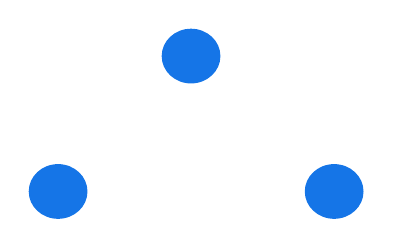
\begin{tikzpicture}[x=0.75pt,y=0.75pt,yscale=-1,xscale=1]
%uncomment if require: \path (0,135); %set diagram left start at 0, and has height of 135

%Shape: Ellipse [id:dp576785563635352] 
\draw  [draw opacity=0][fill={rgb, 255:red, 21; green, 117; blue, 231 }  ,fill opacity=1 ] (88.33,38.19) .. controls (88.33,30.9) and (94.66,25) .. (102.48,25) .. controls (110.29,25) and (116.63,30.9) .. (116.63,38.19) .. controls (116.63,45.47) and (110.29,51.37) .. (102.48,51.37) .. controls (94.66,51.37) and (88.33,45.47) .. (88.33,38.19) -- cycle ;
%Shape: Ellipse [id:dp5059258886052] 
\draw  [draw opacity=0][fill={rgb, 255:red, 21; green, 117; blue, 231 }  ,fill opacity=1 ] (157.27,103.42) .. controls (157.27,96.13) and (163.61,90.23) .. (171.42,90.23) .. controls (179.24,90.23) and (185.58,96.13) .. (185.58,103.42) .. controls (185.58,110.7) and (179.24,116.6) .. (171.42,116.6) .. controls (163.61,116.6) and (157.27,110.7) .. (157.27,103.42) -- cycle ;
%Shape: Ellipse [id:dp140521787960731] 
\draw  [draw opacity=0][fill={rgb, 255:red, 21; green, 117; blue, 231 }  ,fill opacity=1 ] (24.27,103.42) .. controls (24.27,96.13) and (30.61,90.23) .. (38.42,90.23) .. controls (46.24,90.23) and (52.58,96.13) .. (52.58,103.42) .. controls (52.58,110.7) and (46.24,116.6) .. (38.42,116.6) .. controls (30.61,116.6) and (24.27,110.7) .. (24.27,103.42) -- cycle ;




\end{tikzpicture}